\documentclass[a4paper]{article}

%% Language and font encodings
\usepackage{polski}
\usepackage[utf8]{inputenc}
\usepackage[T1]{fontenc}
\usepackage{pdfpages}
\usepackage{indentfirst}
\usepackage{cancel}

% Adjust penalties
\brokenpenalty=1000
\clubpenalty=1000
\widowpenalty=1000

%% Sets page size and margins
\usepackage[a4paper]{geometry}

%% Useful packages
\usepackage{amsmath}
\usepackage{graphicx}
\usepackage[colorlinks=true, allcolors=blue]{hyperref}
\usepackage{booktabs}
\usepackage{ulem}
\usepackage{tikz}

\usepackage{float}

\renewcommand\thesection{\arabic{section}.}
\renewcommand\thesubsection{\arabic{section}.\arabic{subsection}.}
\renewcommand\thesubsubsection{\arabic{section}.\arabic{subsection}. \arabic{subsubsection}.}

% The following commands are not supported in PSTricks at present
% We define them conditionally, so when they are implemented,
% this pgf file will use them.
\ifx\du\undefined
  \newlength{\du}
\fi
\setlength{\du}{15\unitlength}

\newcommand{\Vsp}[1]{\vtop to #1 {}}
\newcommand{\Hsp}[1]{\hbox to #1 {}}
\newcommand{\Small}{\scriptsize}

\title{Sprawozdanie nr 5}
\date{}


\begin{document}

\begin{center}
\begin{tabular}{|p{5.5cm}|l|l|c|}
    \hline
	% Row 1.1  
	    Wydział \Vsp{4mm} &
	    \multicolumn{1}{|l}{Dzień} &
	    poniedziałek $17^{15} - 19^{30}$ &
	    Nr zespołu \\
	% Row 1.2
	    \mbox{\small{Matematyki i Nauk Informatycznych}} &
	    \multicolumn{1}{|l}{Data}  &
	    &
	    \multicolumn{1}{c|}{\Large{18}} \\
    
    \hline
	% Row 2.1 
	    Nazwisko i Imię: &
	    \Small Ocena z przygotowania &
	    \Small Ocena ze sprawozdania &
	    \Small Ocena Końcowa \\
	% Rows 2.2-2.4
	    1. Jasiński Bartosz & & &\\
	    2. Sadłocha Adrian & & & \\
	    3. Wódkiewicz Andrzej & & & \\

    \hline
    % Row 3.1
	    \multicolumn{2}{|l|}{Prowadzący \Vsp{4mm}} &
	    \multicolumn{2}{|l|}{Podpis prowadzącego} \\  
    % Row 3.2
    	\multicolumn{2}{|l|}{} &
    	\multicolumn{2}{|l|}{} \\    	
    \hline
\end{tabular}
\label{pieczatka}
\end{center}

{\let\newpage\relax\maketitle}  % stolen from: https://tex.stackexchange.com/questions/86249/maketitle-text-before-title
\setcounter{secnumdepth}{2}


\section{Opis ćwiczenia}
Ćwiczenie złożone było z następujących części:
\begin{enumerate}
	\item{Badanie prawa Malusa}
	\item{Badanie prawa Snella}
	\item{Wyznaczenie kąta granicznego}
	\item{Wyznaczenie kąta Brewstera}
\end{enumerate}

\subsection{Wstęp teoretyczny}
\subsection{Układ pomiarowy}



\section{Pomiary i obliczenia}
\subsection{Badanie prawa Malusa}
Przy pomocy obu polaryzatorów oraz fotodetektora została zmierzona wartość natężenia światła spolaryzowanego.
Wpierw odnaleziony został taki kąt obrotu analizatora, przy którym mierzona wartość natężenia światła była maksymalna ($\alpha_0 = 176^\circ$).
Następnie, siedmiokrotnie dokonano obrotu analizatora o $15^\circ$ i pomiaru wartości natężenia.
Wyniki zostały przedstawione w tablicy \ref{malus-pomiary}. 
% Pomiary 1. i 7. zostały uznane jako błędy grube na podstawie próby dopasowania wykresu funkcji $263 \cos^2(x+10)$ do wyników pomiarów (patrz rysunek \ref{malus-wykres}).
Na rysunku \ref{malus-wykres} przedstawione zostały 2 próby jak najlepszego dopasowania wykresu funkcji $\cos^2$ uwzględniając wszystkie niepewności standardowe, przy założeniach:
\begin{itemize}
	\item kąt $\alpha_0$ jest kątem, dla którego natężenie jest maksymalne -- kolor czerwony
	\item kąty obrotu analizatora zostały odczytane z przesunięciem $10^\circ$, pomiar $k=1$ jest błędem grubym, a kąt $\alpha_0$ \textbf{nie} jest kątem maksymalnego natężenia -- kolor zielony
\end{itemize}

Biorąc pod uwagę trudności podczas przeprowadzania ćwiczenia, pomimo większej ilości założeń prawdziwy zdaje się być przypadek drugi (kolor zielony na wykresie).


\begin{table}[h]
\centering
\begin{tabular}{rrrr}
\toprule
 $k$ &  $\alpha_k \ ({}^\circ)$ &  $I \ (\mu\text{A})$ &  $u_I \ (\mu \text{A})$ \\
\midrule
 0 &       176 &   260.0 &         3.662877 \\
 \textit{1} & 	   \textit{161} &   \textit{240.0} &         \textit{3.662877} \\
 2 &       146 &   225.0 &         3.662877 \\
 3 &       131 &   160.0 &         3.662877 \\
 4 &       116 &    94.0 &         1.414214 \\
 5 &       101 &    32.0 &         1.414214 \\
 6 &        86 &     2.2 &         0.036629 \\
 7 &        71 &    13.0 &         0.366288 \\
\bottomrule
\end{tabular}
\caption{Pomiary natężenia światła spolaryzowanego}
\label{malus-pomiary}
\end{table}



\begin{figure}[h]
\centering
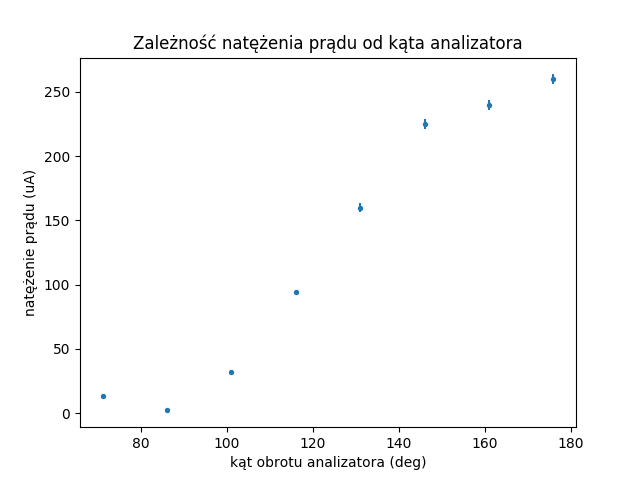
\includegraphics[scale=0.6]{malus.png}
\caption{Prawo Malusa}
\label{malus-wykres}
\end{figure}


\subsection{Badanie prawa Snella}

\begin{figure}[h]
\centering
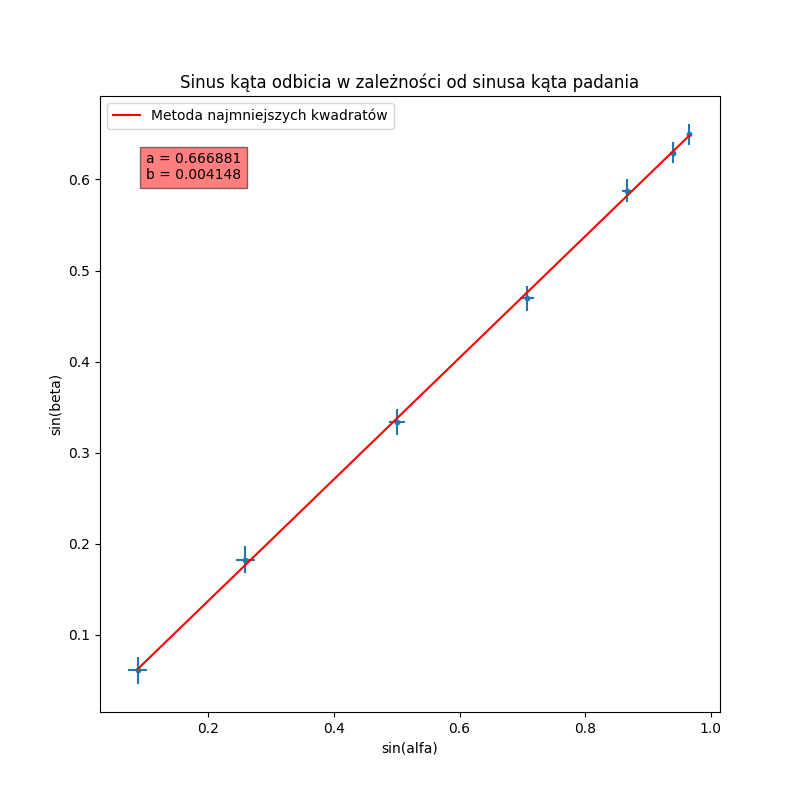
\includegraphics[scale=0.7]{snell.png}
\caption{Wykres }
\end{figure}


\subsection{Wyznaczenie kąta granicznego}
\subsection{Wyznaczenie kąta Brewstera}


\subsection{Wnioski}


\end{document}
